\section{倾角影响}
\label{sec:3.2}

本节从计算射线在某些理想条件下的旅行时间来开始地震旅行时间对炮检距依赖关系的
研究。

\subsection{平面反射面情形下的剖面与道集}
\label{sec:3.2.1}

对于反射资料,最简单情况就是如图\ref{fig:ofs/twopoint}所示的一个水平反射分界面。正如所预料的,
零炮检距剖面酷似地层模型。共中心点道集的时距曲线是双曲线,其渐近线是直线,该直线
的斜率等于速度$v_1$的倒数。最基本的数据处理称为共深度点叠加。即CDP叠加。处理中,
将典中心点道集(CMP)的所有记录道进行时差校正,使时距曲线拉平成为直线,然后彼
此相加,所得结果酷似一个零炮检距记录道。所有这些记录道集合起来,就叫作共深度点叠
加剖面。实际上,总是把CDP叠加剖面当作是一个零炮检距剖面来加以解释和进行偏移.
在本节中,我们将要讨论如何避免采用这种流行的、过于简单化的假设。

\begin{figure}[H]
\centering
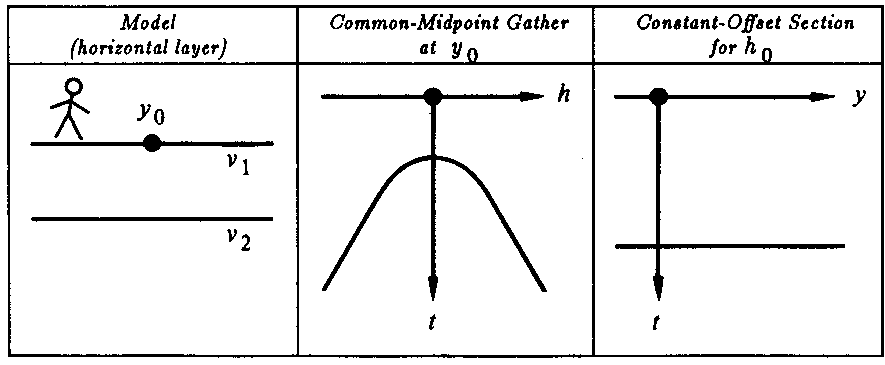
\includegraphics[width=0.65\textwidth]{ofs/simple}
\caption[simple]{最简单的地层模型}
\label{fig:ofs/simple}
\end{figure}

其次一种最简单情形是具有平面反射面,但方向为垂直而非水平。这种情形并不是典型
情形,不过因为地层倾角的影响在极端情形下更易被理解,所以讨论中还是包括了这种情
形。现在,波是沿着空气与大地的分界面传播.为避免混乱,可令反射面以很小的角度偏离
垂直方向,如图\ref{fig:ofs/vertlay}所示。

\begin{figure}[H]
\centering
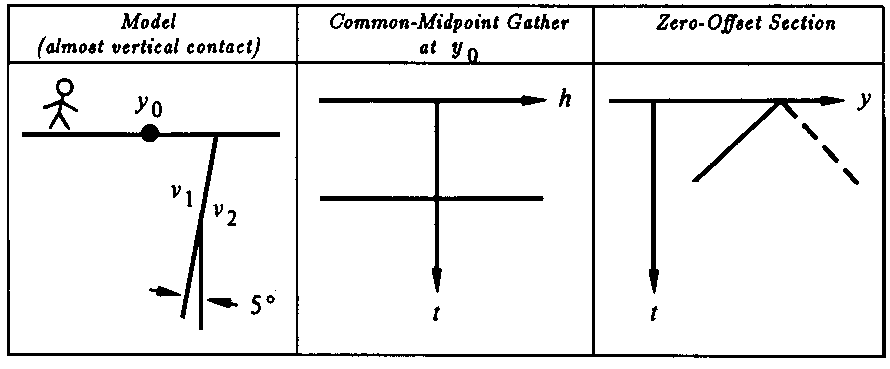
\includegraphics[width=0.65\textwidth]{ofs/vertlay}
\caption[vertlay]{将近垂直的反射面以及相应的道集和剖面}
\label{fig:ofs/vertlay}
\end{figure}

图\ref{fig:ofs/vertlay}表明,旅行时间并不随炮检距之改变而变化。当炮点与检波点彼此逐渐分离
时,旅行时间并不随之增加,看起来似乎有些自相矛盾,解释这种矛盾的关键就在于:保
持恒定不变的是中心点,而不是炮点。在炮检距增大时,炮点虽越易远离该反射面而检波点
却更接近于该反射面,因而,在一个射线路程上的时间减小了,在另一个路程上的时间却增
大了。

平面反射面可以具有位于水平与垂直之间的任何倾角,从而其共中心点道集应处于图
\ref{fig:ofs/twopoint}所示共中心点道集与图\ref{fig:ofs/vertlay}那种共中心点道集之间。
图\ref{fig:ofs/vertlay}内的零炮检距剖面是一条直线,原来它就是双曲线族的渐近线,该渐近线的斜率就等于速度$v_1$的倒数。

\subsection{倾斜层}
\label{sec:3.2.2}

尽管倾斜层形成的时距曲线很简单,要导出它可并不简单。在导出之前,将先说明一下其
结果:对于一个与水平方向呈$\alpha$角度倾斜的地层,其时距曲线为
\begin{equation}
t^2v^2=4(y-y_0)^2sin^2\alpha+4h^2cos^2\alpha
\label{eq:ex3.2.1}
\end{equation}
在$\alpha=45°$情形下,方程\ref{eq:ex3.2.1}是熟悉的毕达哥拉斯(Pythagoras )锥面,它正好像是
$t^2=z^2+x^2$。对于其他的$\alpha$值,该方程仍然是某种锥面,不过是不大熟悉的一种锥面,因为
轴拉长了。

对于$(h,t)$空间内在$y=y_1$点上的共中心点道集,方程\ref{eq:ex3.2.1}看起来如像$t^2=t_0^2+4h^2/v_{apparent}^2$
。所以,不论地层的倾角$\alpha$如何,共中心点道集总是相当于一种严格的双曲线的。倾
角的影响表现在使双曲线之渐近线改变,从而也就是改变着视速度。这个结论在实际工作中
有着重大意义,并以Levin倾角校正而知名(1971 ):
\begin{equation}
v_{apparent}=v_{earth}/cos(\alpha)
\label{eq:ex3.2.2}
\end{equation}
总而言之,倾角使叠加速度増大了。

图\ref{fig:ofs/dipray}表示共中心点道集的若干射线。注意,各条射线是在不同的地点入射在倾斜地
层上。所以,共中心点道集并不就是共深度点道集。要理解为何反射点在反射面上出现移
动,就得回想一下一项基本几何事实,即三角形中的角平分线一般是并不平分对边的。随着
炮检距增大,反射点就向上倾方向移动。

\begin{figure}[H]
\centering
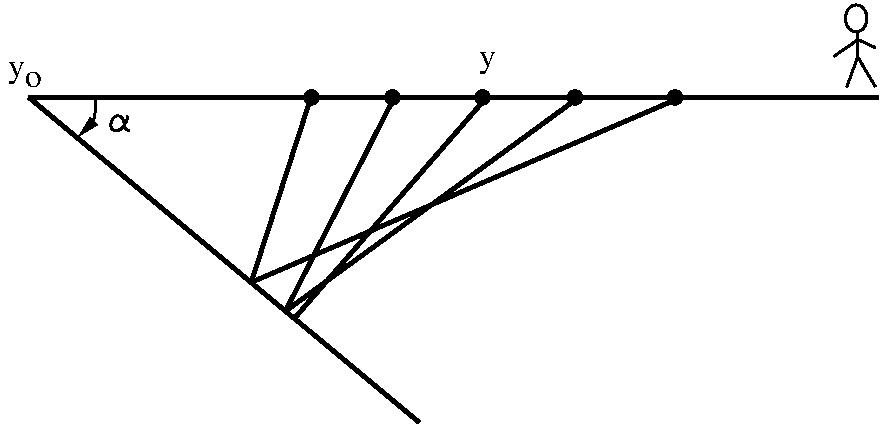
\includegraphics[width=0.65\textwidth]{ofs/dipray}
\caption[dipray]{共中心点道集的射线}
\label{fig:ofs/dipray}
\end{figure}

最后,证明一下式\ref{eq:ex3.2.1}。图\ref{fig:ofs/lawcos}表示的是与位于两倍倾角的另一反射面上的
“虚”震源有关的基本几何关系;为求方便起见,令地层与地面在点相交。根据三角
学的余弦定律可决定图\ref{fig:ofs/lawcos}中的直线之长度为
\begin{figure}[H]
\centering
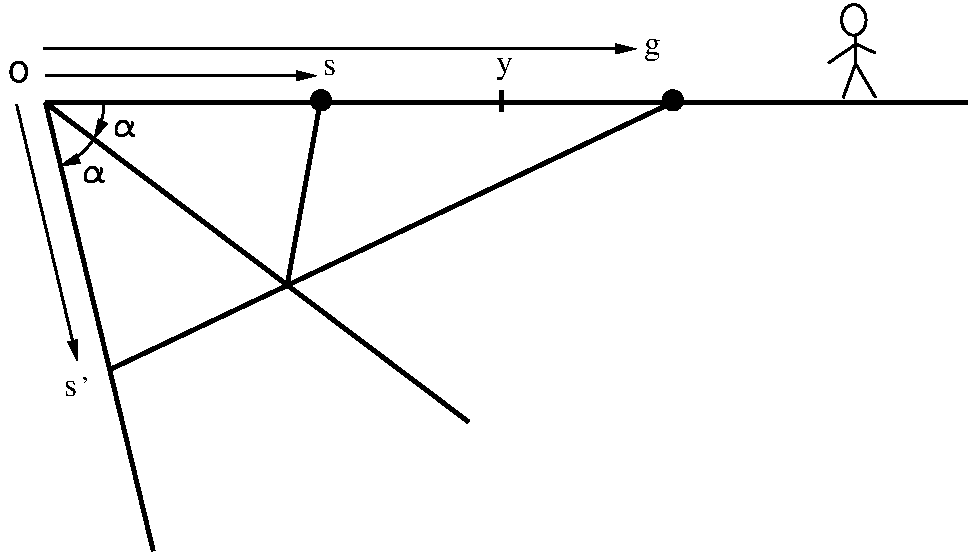
\includegraphics[width=0.65\textwidth]{ofs/lawcos}
\caption[lawcos]{由s'点处之虚震源至g点的旅行时间可用余弦定律表示}
\label{fig:ofs/lawcos}
\end{figure}
\begin{gather*}
t^2v^2=s^2+g^2-2sgcos2\alpha
t^2v^2=(y-h)^2+(y+h)^2-2(y-h)(y+h)cos2\alpha
t^2v^2=2(y^2+h^2)-2(y^2-h^2)(cos^2\alpha-sin^2\alpha)
t^2v^2=4y^2sin^2\alpha+4h^2cos^2\alpha
\end{gather*}
上式就是方程\ref{eq:ex3.2.1}。

式\ref{eq:ex3.2.1}的另一层意思就是:它所描述的是恒定炮检距剖面。出人意外,一个倾斜
的平面地层的旅行时间关系竟在非零炮检距上变得很弯曲——它变成太过分的双曲线了。

\subsection{点源响应}
\label{sec:3.2.3}

另一种简单几何关系是一个反射点位于地层之内时的情形。一个波从任何方向入射在该
点上,将沿所有的方向发生波的反射,由于任何模型都是这类点散射的一种叠加结果,所以这
种几何关系特别重要。图\ref{fig:ofs/twopoint}所示是一个例子。该图中的曲线包括有平点(flat spots),以
这种现象同图\ref{fig:ofs/simple}和图\ref{fig:ofs/vertlay}中的某些曲线呈直线形式是出于相同的原因。
\begin{figure}[H]
\centering
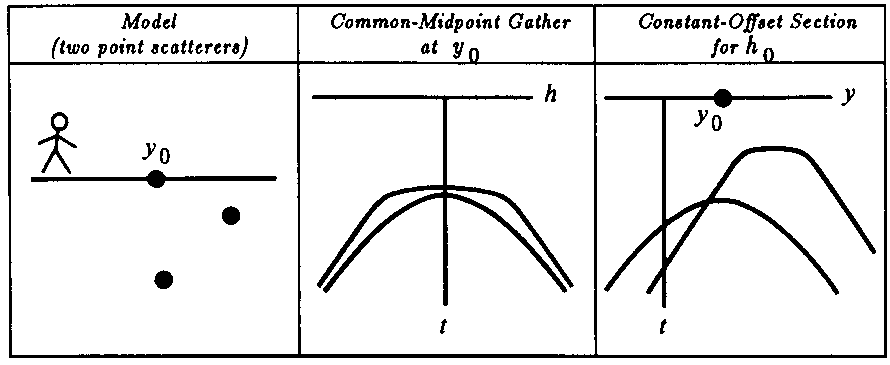
\includegraphics[width=0.65\textwidth]{ofs/twopoint}
\caption[twopoint]{两个点散射之响应。注意图中的平点}
\label{fig:ofs/twopoint}
\end{figure}